\section{Cenário de Teste 3}

Este cenário está dividido em 5 (cinco) exemplos, os quais são apresentados a seguir, contemplando todo o processo de auto-localização
em cada exemplo, a partir da apresentação das Imagens abaixo.

\subsection{Exemplo 1}

Exemplo utilizando velocidade de deslocamento em 2 unidades de diâmetro por segundo:

{\centering
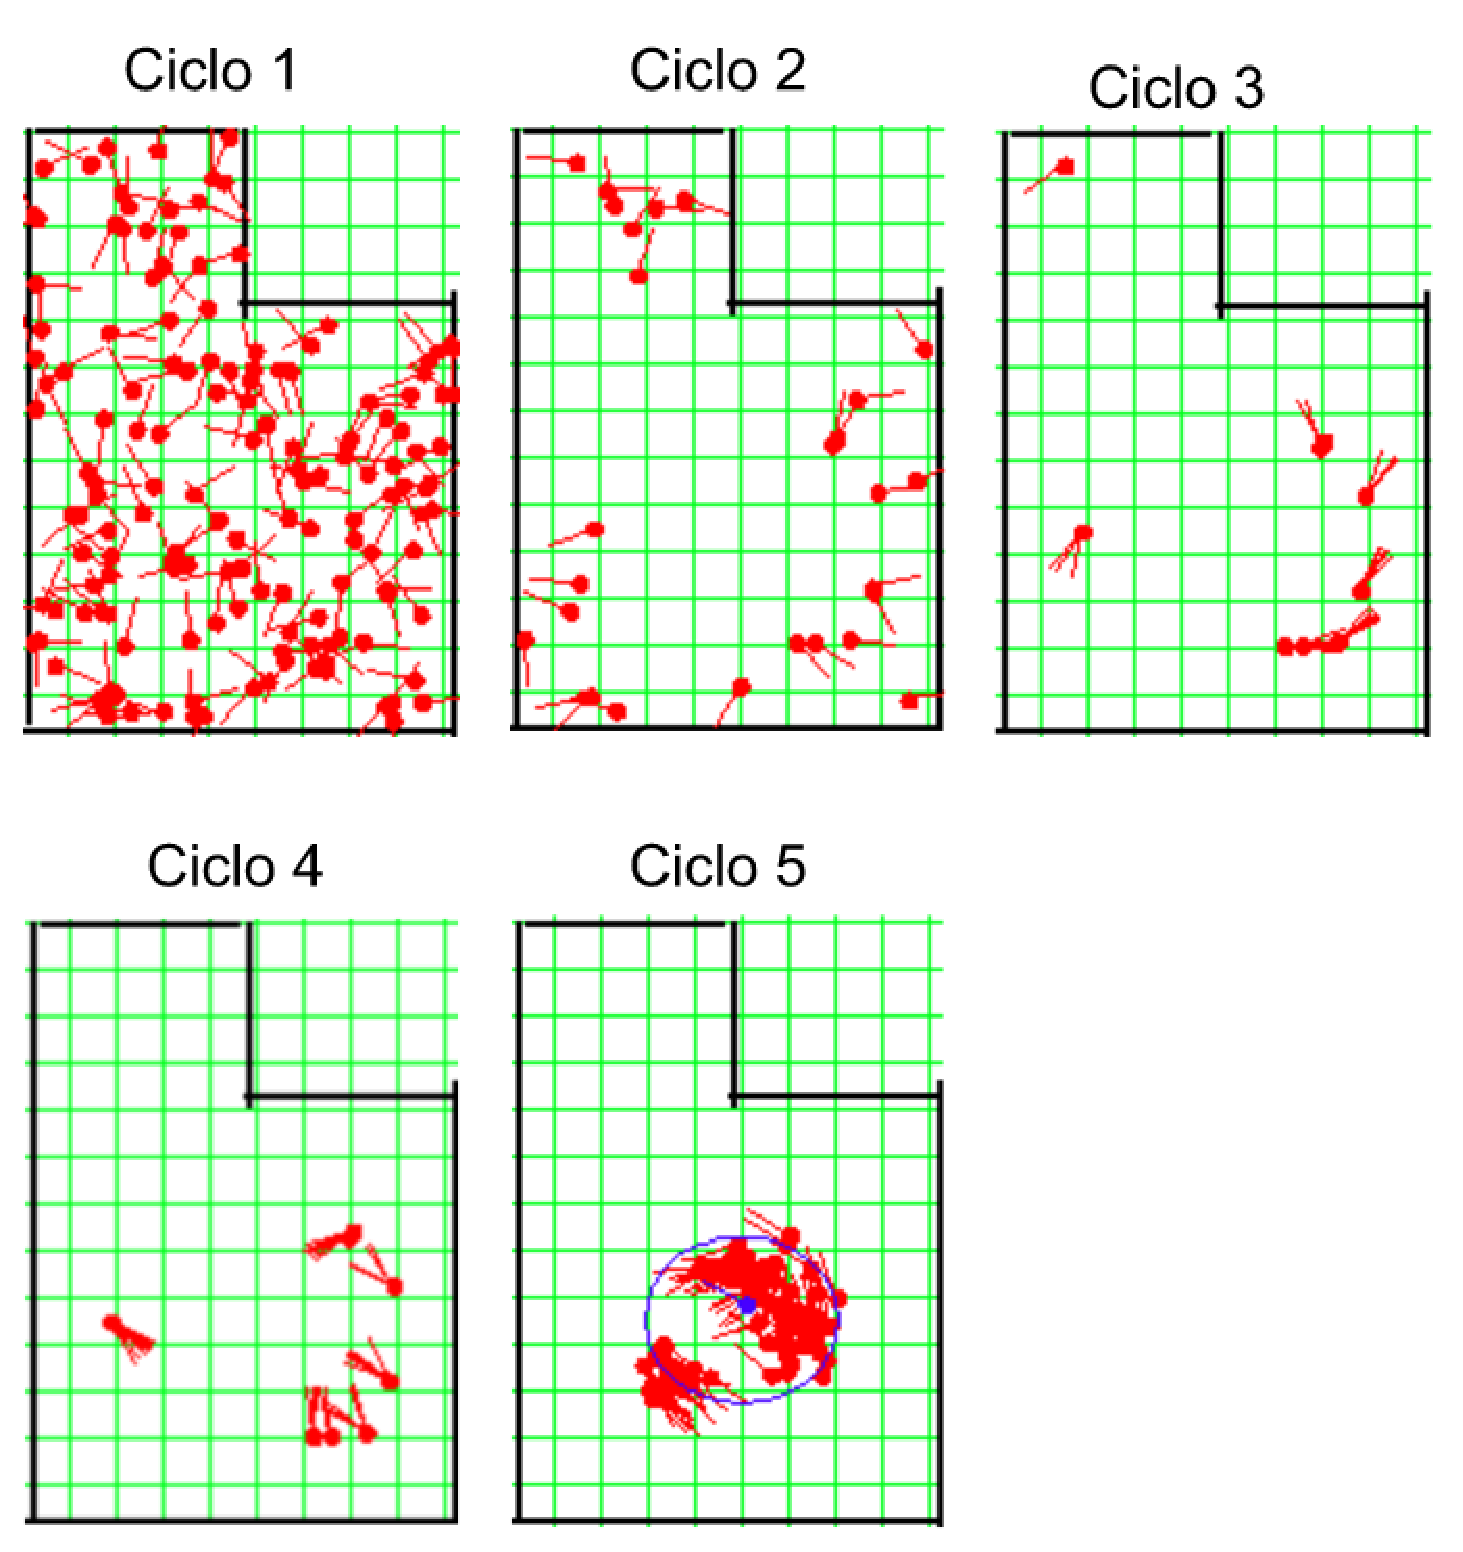
\includegraphics[scale=0.4]{figuras/cen3_ex1.eps}
\captionof{figure}{Cenário 3 - Exemplo 1}
\label{img:cen3_ex1}
\par}


\subsection{Exemplo 2}

Exemplo utilizando velocidade de deslocamento em 5 unidades de diâmetro por segundo:

{\centering
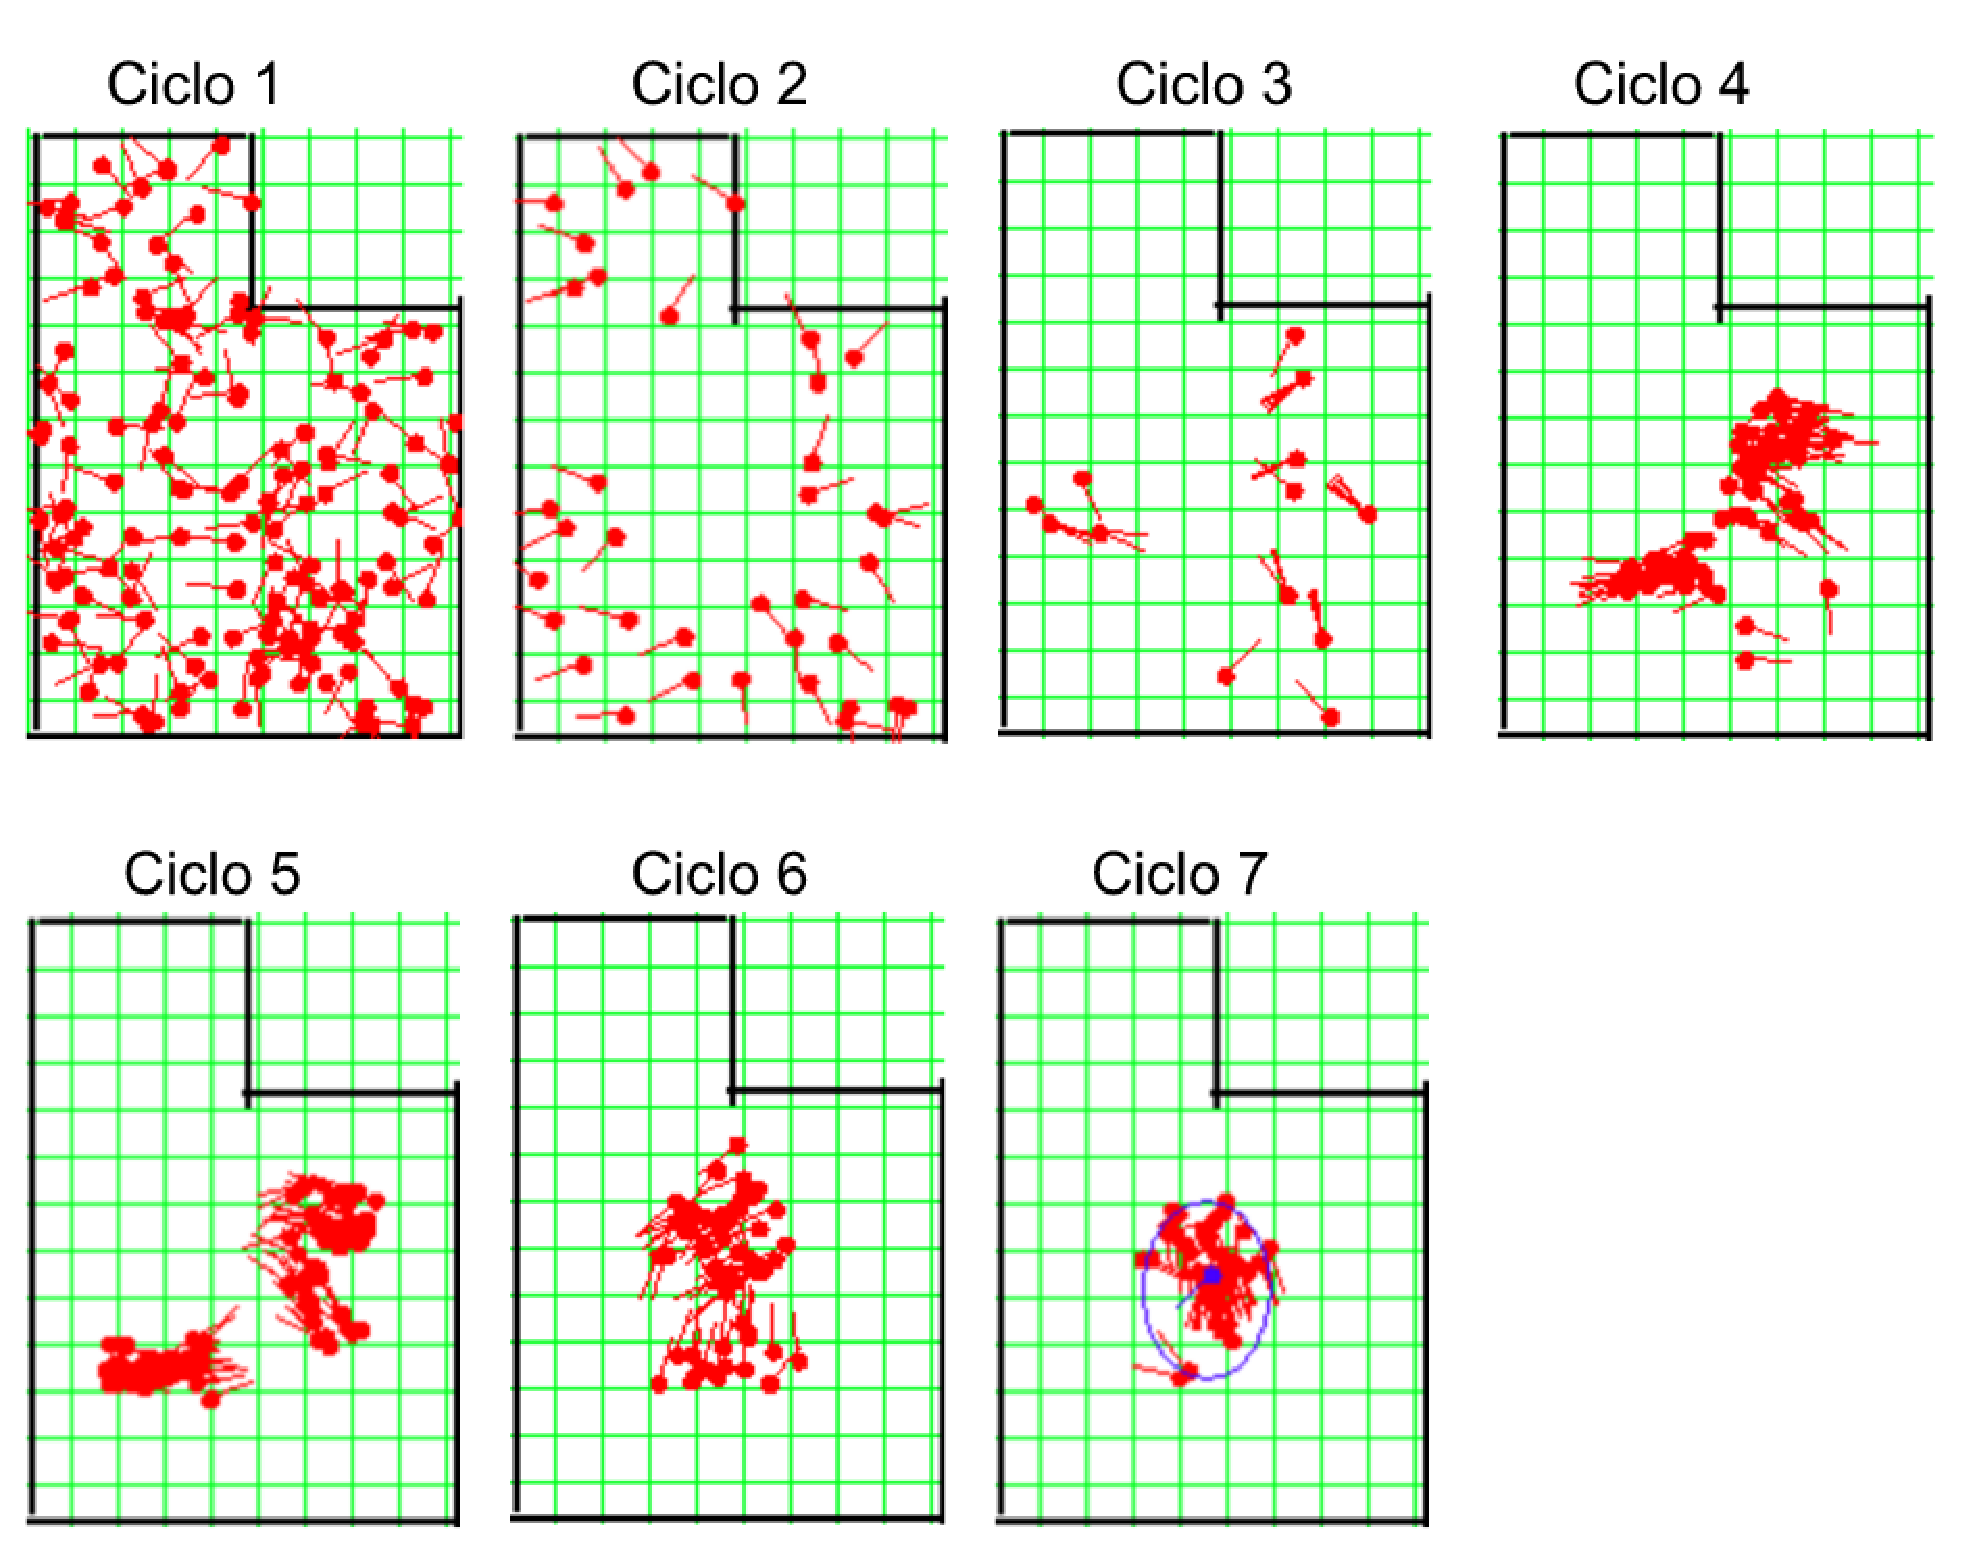
\includegraphics[scale=0.4]{figuras/cen3_ex2.eps}
\captionof{figure}{Cenário 3 - Exemplo 2}
\label{img:cen3_ex2}
\par}


\subsection{Exemplo 3}

Exemplo utilizando velocidade de deslocamento em 10 unidades de diâmetro por segundo:

{\centering
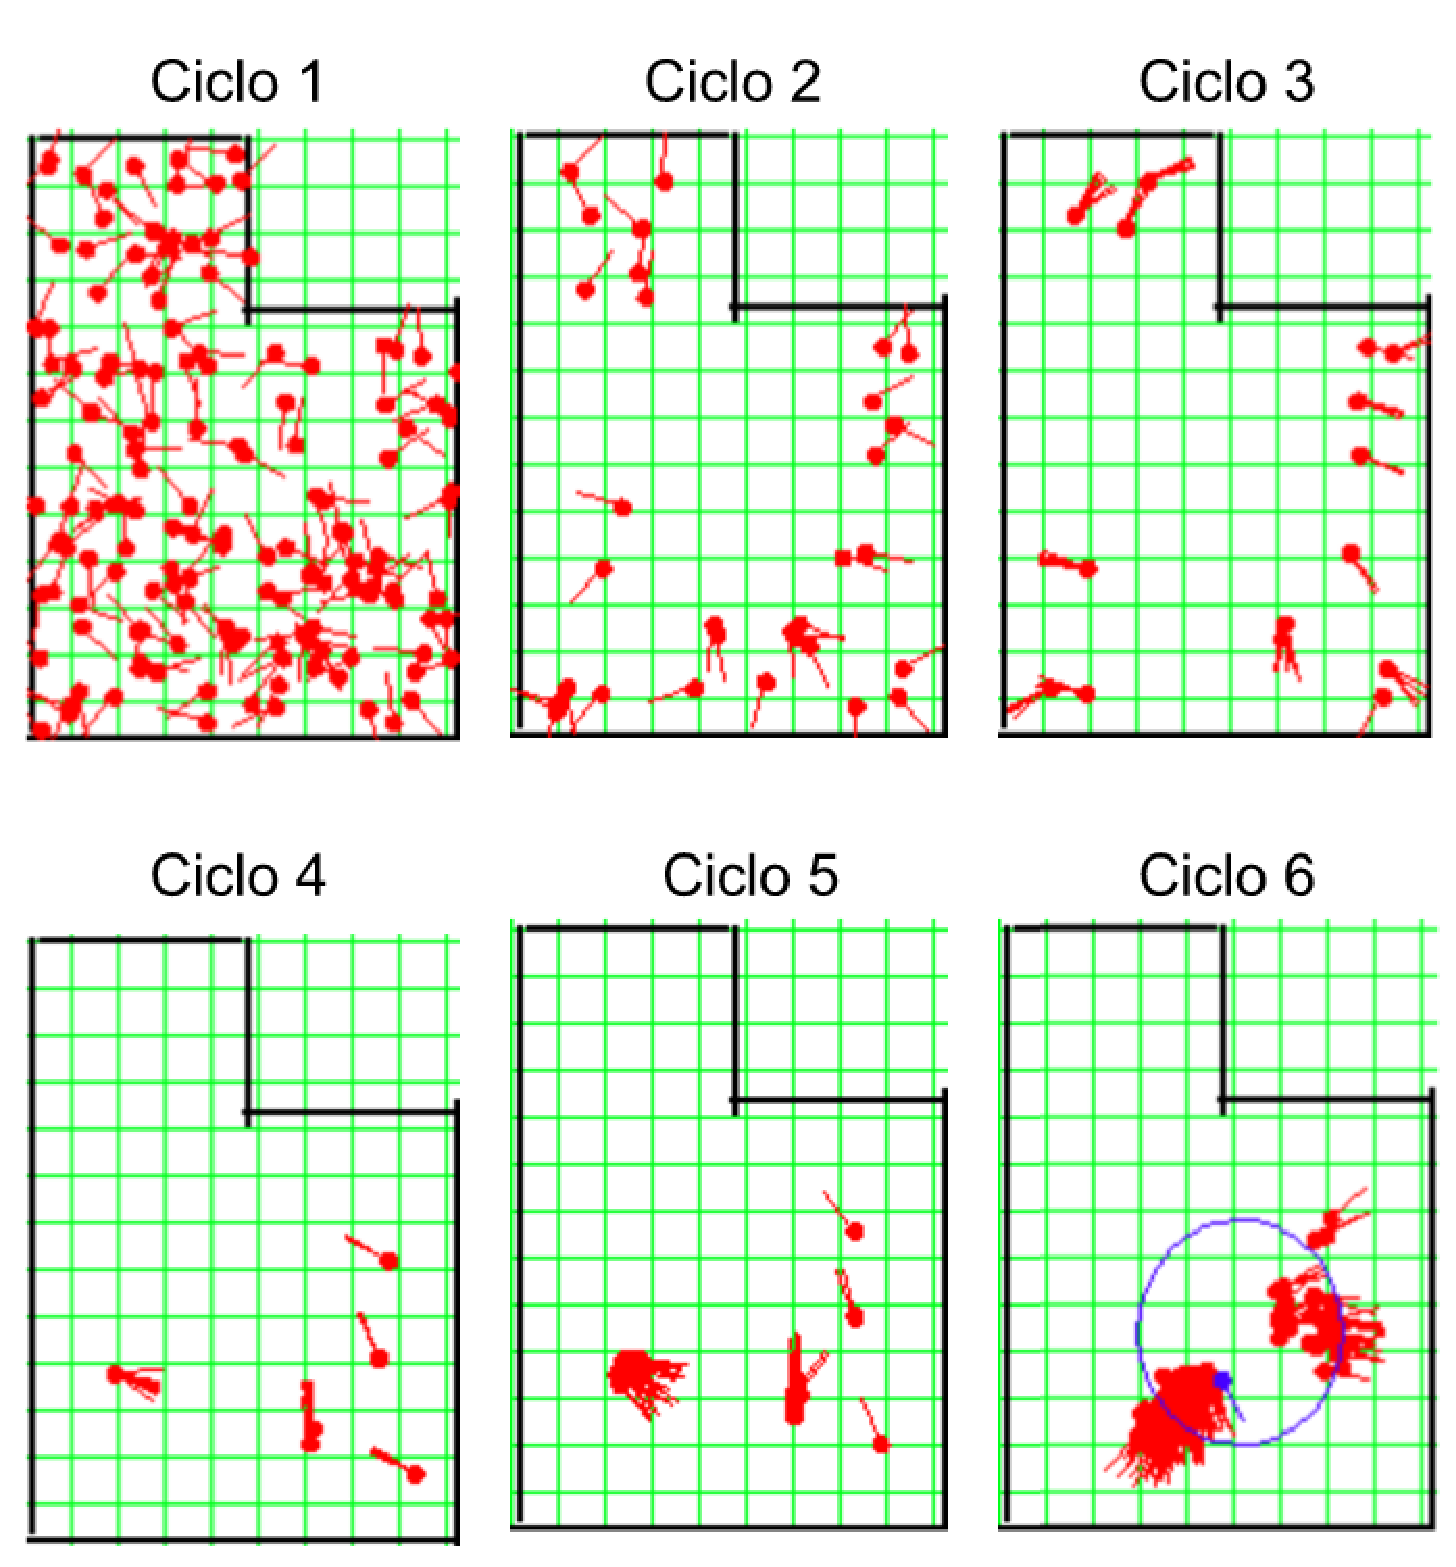
\includegraphics[scale=0.4]{figuras/cen3_ex3.eps}
\captionof{figure}{Cenário 3 - Exemplo 3}
\label{img:cen3_ex3}
\par}

\subsection{Exemplo 4}

Exemplo utilizando velocidade de deslocamento em 15 unidades de diâmetro por segundo:

{\centering
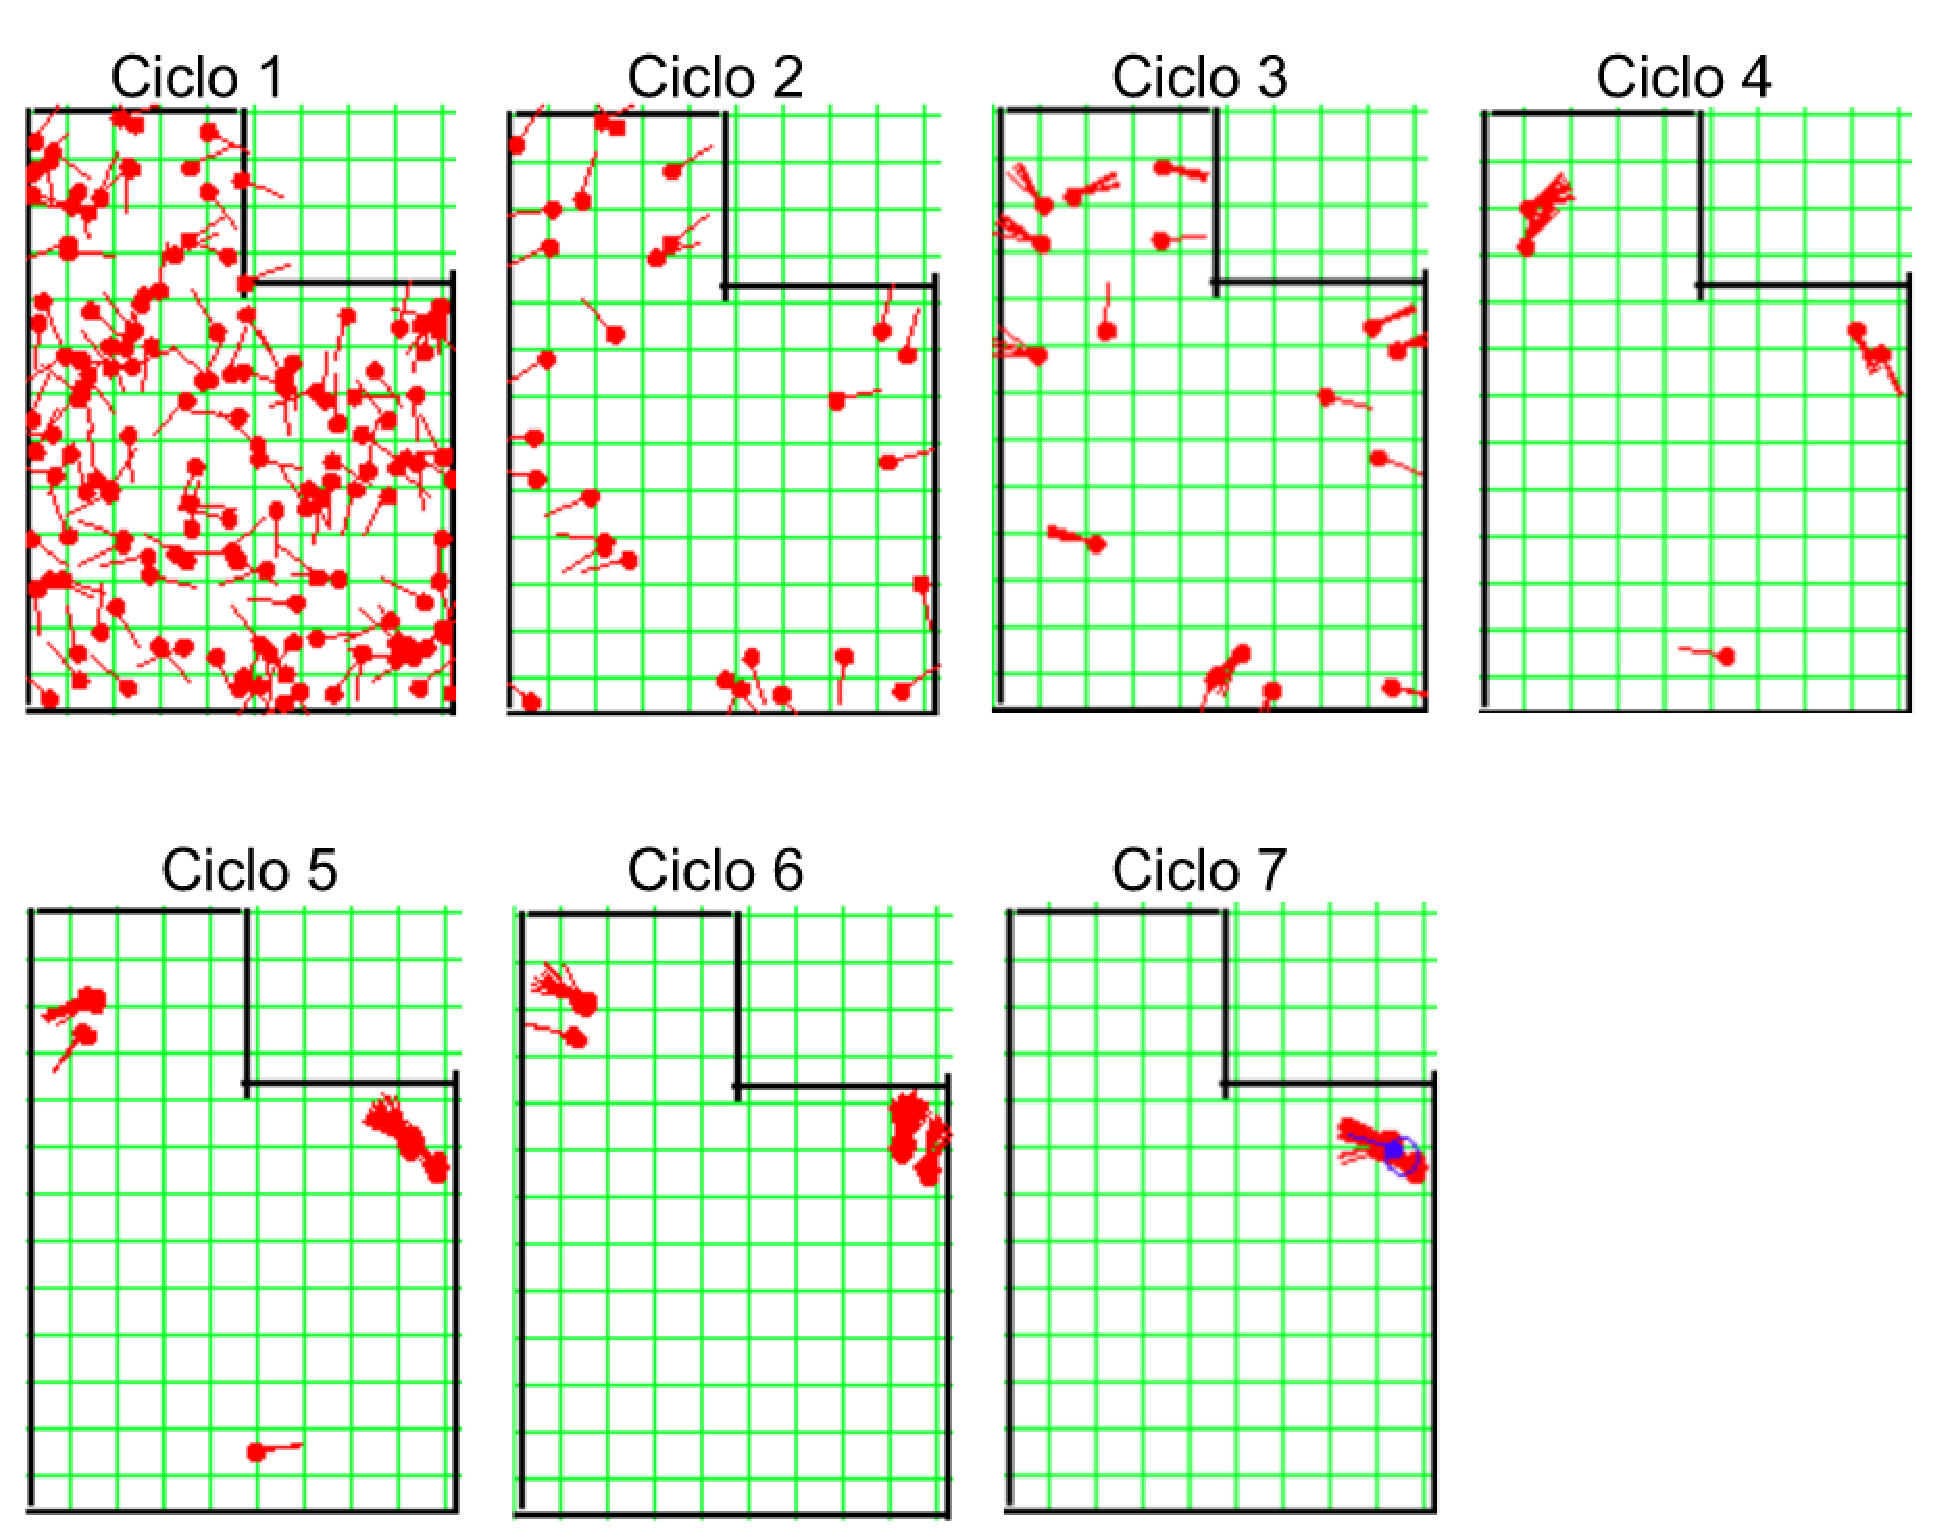
\includegraphics[scale=0.4]{figuras/cen3_ex4.eps}
\captionof{figure}{Cenário 3 - Exemplo 4}
\label{img:cen3_ex4}
\par}

\subsection{Exemplo 5}

Exemplo utilizando velocidade de deslocamento em 30 unidades de diâmetro por segundo:

{\centering
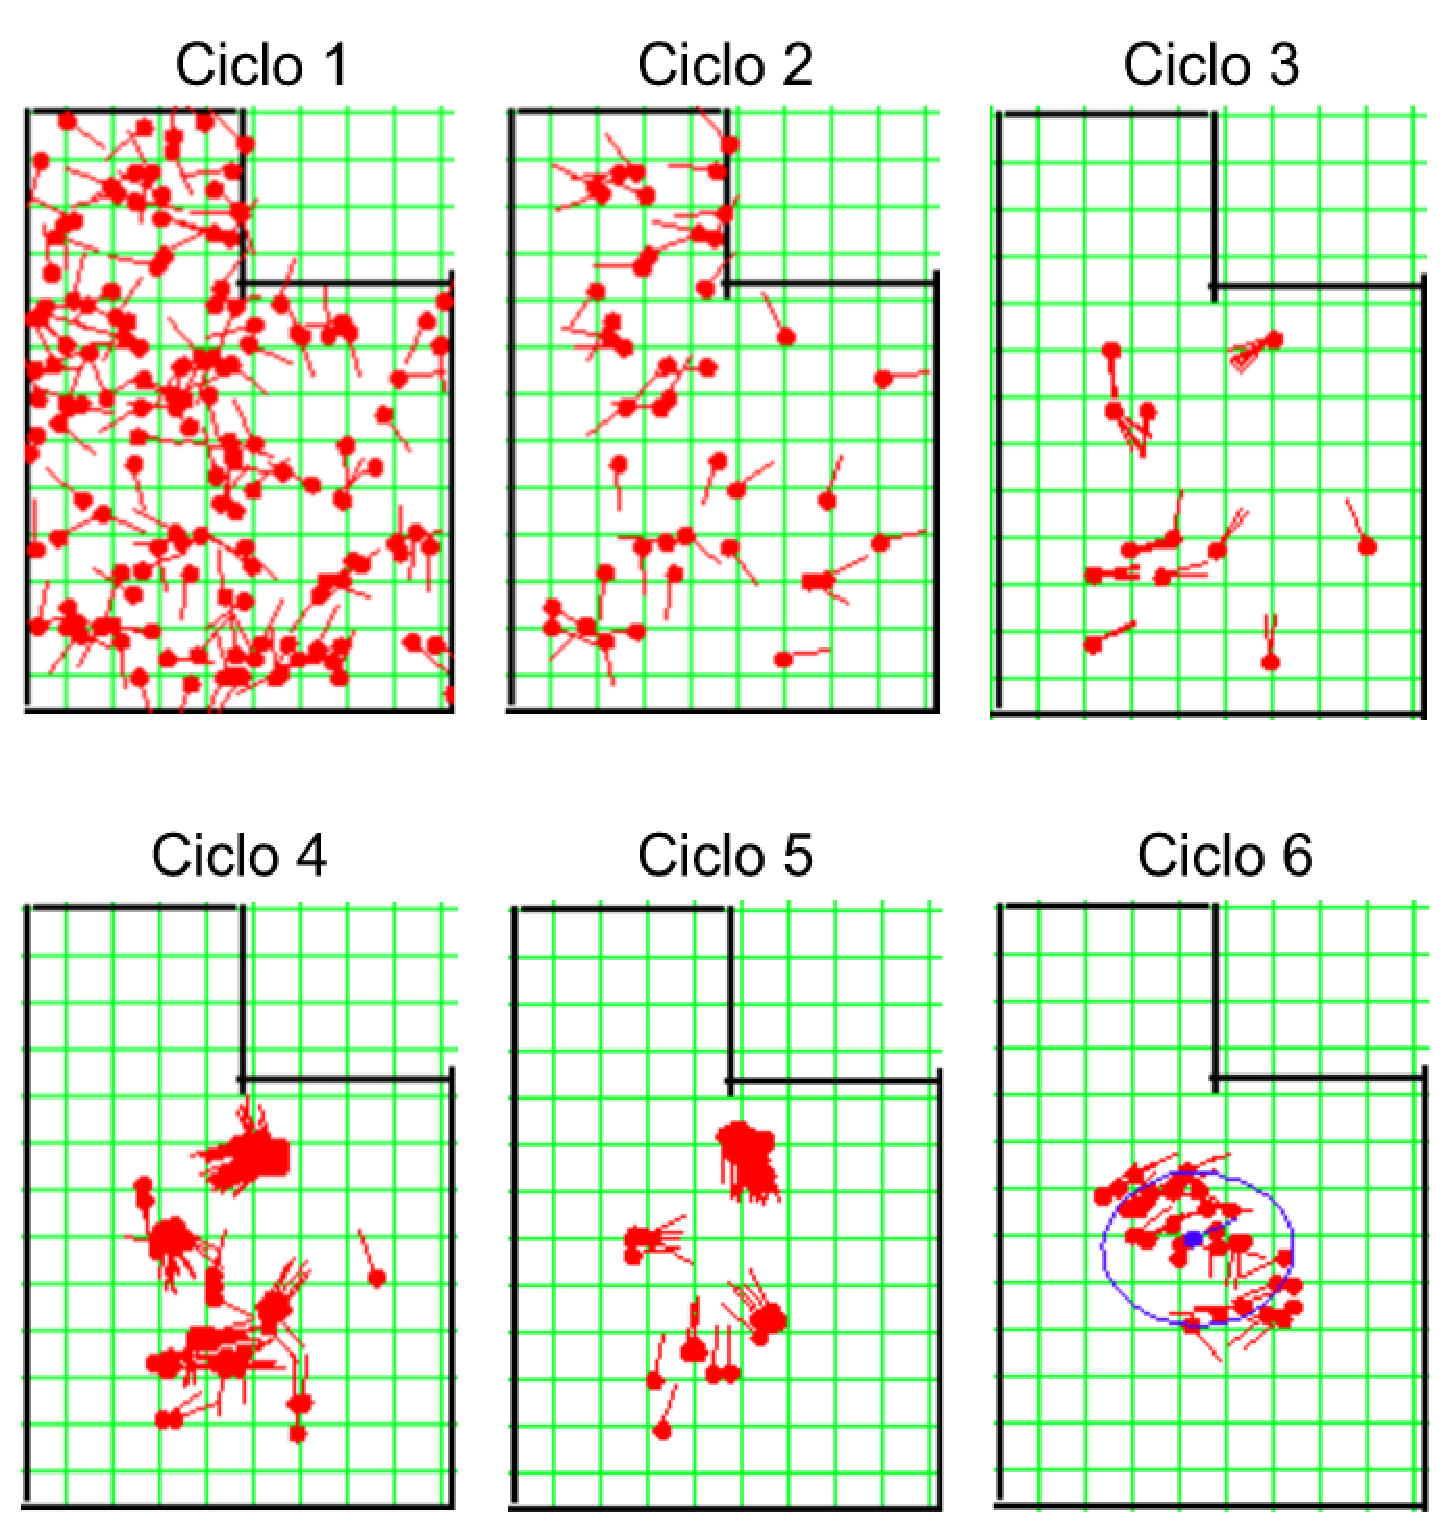
\includegraphics[scale=0.4]{figuras/cen3_ex5.eps}
\captionof{figure}{Cenário 3 - Exemplo 5}
\label{img:cen3_ex5}
\par}
